% -------------------------------------------------------------------------------
% This document provides a template for a text document in the style of the 
% University of Waterloo, Waterloo, Canada.
%
% The LaTeX template is released under the GNU Lesser General Public License. 
% The following applies:
% The LaTeX template is free software: you can redistribute it and/or modify
% it under the terms of the GNU Lesser General Public License as published by
% the Free Software Foundation, either version 3 of the License, or
% (at your option) any later version.
%
% The LaTeX template is distributed in the hope that it will be useful,
% but WITHOUT ANY WARRANTY; without even the implied warranty of
% MERCHANTABILITY or FITNESS FOR A PARTICULAR PURPOSE. See the
% GNU Lesser General Public License for more details.
%
% You should have received a copy of the GNU Lesser General Public License
% along with the JAMS Python package (cf. gpl.txt and lgpl.txt).
% If not, see <http://www.gnu.org/licenses/>.
%
% Copyright 2016-2016 Juliane Mai
% -------------------------------------------------------------------------------
\documentclass{article}

% ----------------------------------------------
% import some additional packages
% ----------------------------------------------
\usepackage{hyperref}
\usepackage{lipsum}                     % to generate some text (only needed in a template)
%\usepackage[german,ngerman]{babel}      % special GERMAN hyphenation, quotes, characters, 
%%                                       % dates and labeling like 'Abb.', 'Tabelle', etc.
%\usepackage[utf8]{inputenc}             % translation of GERMAN umlauts in editor to document
\usepackage[english]{babel}             % ENGLISH hyphenation, quotes, dates and labeling like 'Figures', 'Table', etc.
\usepackage{pdfpages}                   % to attach PDFs to the document
\usepackage{cmbright}                	% Font: --- CM-Bright (eigntlich eine Familie)
\usepackage{fancyhdr}
\usepackage{etoolbox}
%\usepackage{geometry}
\usepackage[top=4cm,bottom=3cm,left=3.5cm,right=3.5cm,headsep=1.0in]{geometry} 
\usepackage{xcolor}
\usepackage{varwidth}
\usepackage{lastpage}
\usepackage{textcomp}
\usepackage{graphicx}
\usepackage{multirow}
\usepackage{amsmath}
\usepackage{amssymb}
\usepackage{enumerate}
\usepackage{pdflscape}
\usepackage{textcomp}
\usepackage[width=.9\textwidth]{caption}

\usepackage{array}
\newcolumntype{L}[1]{>{\raggedright\let\newline\\\arraybackslash\hspace{0pt}}m{#1}}
\newcolumntype{C}[1]{>{\centering\let\newline\\\arraybackslash\hspace{0pt}}m{#1}}
\newcolumntype{R}[1]{>{\raggedleft\let\newline\\\arraybackslash\hspace{0pt}}m{#1}}

\usepackage{tikz}
\usetikzlibrary{shapes,decorations,shadows}
\usetikzlibrary{calc}
\usetikzlibrary{fadings}
%\usepgflibrary{arrows}
\usetikzlibrary{arrows}
%\usetikzlibrary{arrows.meta}
\usetikzlibrary{backgrounds}

\setlength{\parindent}{0pt}

\pdfpagewidth=8.5in   % 210mm for A4
\pdfpageheight=11.0in % 297mm for A4

\pagestyle{fancy}
\renewcommand\familydefault{\sfdefault}

\patchcmd{\headrule}{\hrule}{\color{black}\hrule}{}{}
\patchcmd{\footrule}{\hrule}{\color{black}\hrule}{}{}

\fancypagestyle{plain}{
	\fancyhf{}
	\lhead{\textcolor{black}{
\includegraphics[width=4.5cm]{figures/Logo_top}}}
	\chead{\textcolor{black}{}}
	\rhead{\parbox[b][15mm][t]{0.5\textwidth}{\raggedright 
			Department Civil \& Environmental Engineering\\
			Juliane Mai\\
			{\small Phone: +1 (519) 888-4567 Ext. 30016}\\[-2pt]
			{\small E-Mail: juliane.mai@uwaterloo.ca}}
		}
	\rfoot{
\includegraphics[width=2.5cm]{figures/Logo_bottom}}
	\cfoot{\vspace*{-1.4cm}
		Page \thepage\ of \pageref{LastPage}}
	\renewcommand{\footrulewidth}{0.0pt}
	\renewcommand{\headrulewidth}{0.0pt}
}

% ----------------------------------------------
% define UFZ/UW standard colors
% ----------------------------------------------
\definecolor{ufzdarkblue}{RGB}{0,62,110}
\definecolor{ufzblue}{RGB}{0,88,156}
\definecolor{ufzlightblue}{RGB}{0,162,224}
\definecolor{ufzred}{RGB}{212,45,18}
\definecolor{ufzorange}{RGB}{207,104,0}
\definecolor{ufzyellow}{RGB}{230,175,17}
\definecolor{ufzdarkgreen}{RGB}{20,77,40}
\definecolor{ufzgreen}{RGB}{169,181,9}
\definecolor{ufzgray1}{RGB}{81,81,81}
\definecolor{ufzgray2}{RGB}{156,156,156}
\definecolor{ufzgray3}{RGB}{185,185,185}
\definecolor{ufzblack}{RGB}{0,0,0}
\definecolor{ufzwhite}{RGB}{255,255,255}	
\definecolor{uwred}{RGB}{183,18,52}
\definecolor{uwyellow}{RGB}{255,215,79}

\newcommand{\UW}[1]{\textcolor{uwred}{#1}}

\tikzstyle{whitebox} = [rectangle, rounded corners, align=center, minimum width=3cm, minimum height=1cm,text centered, draw=black, fill=ufzwhite!30]
\tikzstyle{emptybox} = [align=center, minimum width=4cm, minimum height=1cm,text centered] %, draw=black]
\tikzstyle{textbox} = [minimum width=4cm, minimum height=1cm,draw=black]

% bibliogrpahy
\usepackage{natbib}
\bibliographystyle{agu/BibTeX/agufull08}

\begin{document}
	
	\pagestyle{plain}
	
	\vspace*{-1.5cm}
	\begin{center}
		\textbf{\LARGE Integrated Modeling Program for Canada IMPC}\\[4pt]
		{\Large --~Project A5: Model-intercomparison over Great Lakes~--}\\[4pt]
		Authors: Juliane Mai (UWaterloo) \& Nicolas Gasset (ECCC-CMC)
	\end{center}

	\section{Forcing dataset}

	The forcing dataset is a subset from a preliminary sample of an atmospheric reforecast and precipitation/land-surface reanalysis dataset that is currently in development at ECCC-CMC~\citep{gasset2017c,gasset2018a}. 
	To obtain such a dataset, as illustrated in Fig.~\ref{fig:reforecast_analysis_system_overview}, ERA-Interim reanalysis data ($\sim 80$~km horizontal resolution)~\citep{dee2011} are used to initialize the so-called Global Deterministic Reforecast System (GDRS). The latter is based on the latest stable version of the Global Environmental Multiscale (GEM, v4.8-LTS) model~\citep{cote1998,cote1998a,girard2013} and feature a global latitude-longitude uniform grid with about $50$~km spatial resolution. 
	Then, following a dynamical downscaling approach, the so-called Regional Deterministic Reforecast System (RDRS) is run. RDRS is also initialized by ERA-Interim but driven by the GDRS. The RDRS is based on the same version of GEM and feature a similar configuration, but the area is limited to a rotated latitude-longitude uniform grid with about $15$~km horizontal resolution that covers whole North America and the Arctic Ocean. Both of these systems- the GDRS and RDRS-  are closely related to the control member of the Global and Regional Ensemble Prediction System (GEPS/REPS)~\citep{charron2009,lavaysse2012,houtekamer2013,gagnon2015,lin2016} which are both operational at ECCC-CMC. Operational means that they have undergone a strict and thorough validation procedure. Both the GDRS and the RDRS are launched twice a day (every 12-h at 0~UTC and 12~UTC) and integrated for 24-h. 
	
%   \begin{figure}[h]
%      \centering
%      \includegraphics[width=0.75\linewidth]{figures/schema_system_nice.png}
%      \caption{Illustration of the atmospheric reforecast and precipitation/land-surface reanalysis system that is currently in development at ECCC-CMC.}
%      \label{fig:reforecast_analysis_system_overview}
%   \end{figure}

	\begin{figure}[h]
		\centering
		\tikzstyle{line} = [draw, -latex']
		\tikzstyle{arrow} = [thick,->,>=stealth, -latex']
		\begin{tikzpicture}[node distance=2.0cm,scale=0.1cm,line width=0.5pt]
		
		\node [emptybox, yshift=0.0] (ERA) {ERA-Interim: \\1979 to today\\ ($\sim 80km/6h$)};
		\node[emptybox, below of=ERA, yshift=-1.0cm] (GEM-Surf) {GEM-Surf (50 km)\\ Surface Model\\[4pt]
			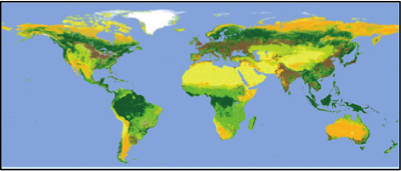
\includegraphics[width=4cm]{figures/GEM-Surf.png}};
		\node[emptybox, right of=ERA, xshift=3.0cm, yshift=-1.0cm] (GEM-GDRS) {GEM GDRS (50 km)\\ Atmospheric Model\\[4pt]
			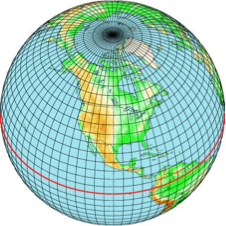
\includegraphics[width=2cm]{figures/GEM-GDRS.png}};
		\node[emptybox, right of=GEM-GDRS, xshift=3.0cm, yshift=0.0cm] (GEM-RDRS) {GEM RDRS (15 km)\\ Atmospheric Model\\[4pt]
			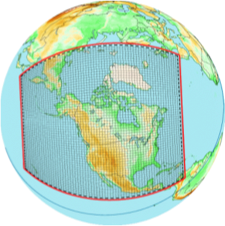
\includegraphics[width=2cm]{figures/GEM-RDRS.png}};
		
		\node[emptybox, below of=GEM-GDRS, xshift=0.0cm, yshift=-3.0cm] (Obs-gray) {Surface Observations\\[4pt]
			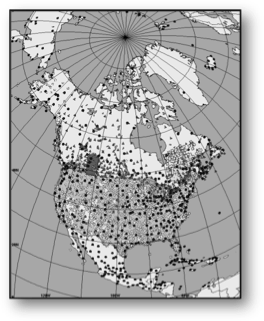
\includegraphics[width=2cm]{figures/Observations_gray.png}};
		\node[emptybox, below of=GEM-RDRS, xshift=0.0cm, yshift=-3.0cm] (Obs) {Surface Observations\\[4pt]
			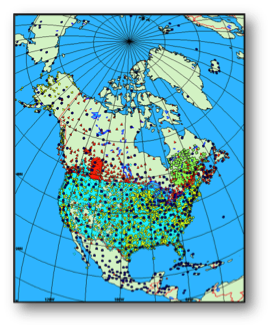
\includegraphics[width=2cm]{figures/Observations.png}};
		
		\node [emptybox, below of=GEM-GDRS, yshift=-0.5cm, xshift=2.5cm] (text) {\textit{Precipitation and surface} \\ \textit{data assimilation:}\\ \textit{CaPA and CaLDAS}};
		
		% Draw edges
		\draw [->,  color=ufzlightblue, line width=3pt, -latex'] (ERA) edge (GEM-Surf);
		\draw [->,  color=ufzblue,      line width=3pt, -latex'] (ERA) edge (GEM-GDRS);
		\draw [->,  color=ufzblue,      line width=3pt, -latex'] (GEM-Surf) edge (GEM-GDRS);
		\draw [->,  color=ufzlightblue, line width=3pt, -latex'] (GEM-GDRS) edge (GEM-RDRS);
		\draw [<->, color=ufzgray2,     line width=3pt, latex'-latex'] (GEM-GDRS) edge (Obs-gray);
		\draw [<->, color=ufzdarkblue,  line width=3pt, latex'-latex'] (GEM-RDRS) edge (Obs);
		
		% Legend
		\draw [-latex',       color=ufzlightblue,  line width=3pt] (-0.7,-2.00) -- (-0.3,-2.00);
		\draw [-latex',       color=ufzblue,       line width=3pt] (-0.7,-2.15) -- (-0.3,-2.15);
		\draw [latex'-latex', color=ufzdarkblue,   line width=3pt] (-0.7,-2.30) -- (-0.3,-2.30);
		\node[draw=white,text width=4cm, align=left] at (0.5,-2.00) {Initialization + forcing};
		\node[draw=white,text width=4cm, align=left] at (0.5,-2.15) {Initialization};
		\node[draw=white,text width=4cm, align=left] at (0.5,-2.30) {Assimilation};
		\end{tikzpicture}
		\caption{Illustration of the atmospheric reforecast and precipitation/land-surface reanalysis system that is currently in development at ECCC-CMC.}
		\label{fig:reforecast_analysis_system_overview}
	\end{figure}
   
	Surface initial conditions such as sea surface temperature, sea ice concentration/thickness, soil moisture, soil temperature and snowpack conditions that are consistent with the driving data and the surface scheme of GEM are additionally  required as input of the GDRS and RDRS.
	%Surface initial condition (sea surface temperature, sea ice concentration/thickness, soil moisture, soil temperature and snowpack conditions) consistent with the surface scheme included in GEM also need to be provided. 
	For the GDRS, they are obtained from an a priori 30 years off-line (open-loop) simulation of GEM land-surface model GEM-Surf \citep{carrera2010,bernier2012} on the same grid as the GDRS and directly forced by the near-surface fields of ERA-Interim reanalysis as well as the 3-hour precipitation amounts~\citep{gagnon2015}.
	This off-line system includes a land-surface scheme, i.e., ISBA \citep{noilhan1989,noilhan1996}, as well as a sea ice and a glacier scheme which are part of the GEM model itself. 
	For the RDRS, the surface initial fields are obtain though a coupling with the Canadian Land Data Assimilation System (CaLDAS)~\citep{balsamo2007,carrera2015} which include the Canadian Precipitation Analysis (CaPA) system~\citep{mahfouf2007,lespinas2015} to feed the Ensemble Kalman Filter (EnKF) members with 6-h precipitation analysis. Such an approach have been shown to notably improve surface results compared to the ECCC-CMC operational deterministic approaches for the years 2010-2014~\citep{gasset2018a}. It allows to produce more representative reforecast and precipitation/ land-surface retrospective analysis consistent in time and space at a higher resolution than current reanalysis dataset.
	
	In addition to the above described approach, CaPA is also run in an a posteriori manner to produce 24-h precipitation analysis at 12 UTC relying on the GDRS and RDRS precipitation accumulation as background field. This allows including additional observation datasets, such as data in the Standard Hydrological Exchange Format (SHEF)~\citep{bissell1984}, that only report 24-h accumulation. It also enables the assimilation of the so-called Adjusted Daily Rain and Snow (AdjDlyRS) observations dataset~\citep{wang2017} which is part of the Adjusted and Homogenized Canadian Climate Data (AHCCD). This newly released dataset covering only Canada features one of the most advanced quality control and bias correction procedures allowing, e.g., mitigating under-catchments of solid precipitation in the winter~\citep{wang2017}. The inclusion of such a dataset has also been proven to improve notably results where stations are present~\citep{gasset2018a}.
	
	\begin{figure}[h]
		\centering
		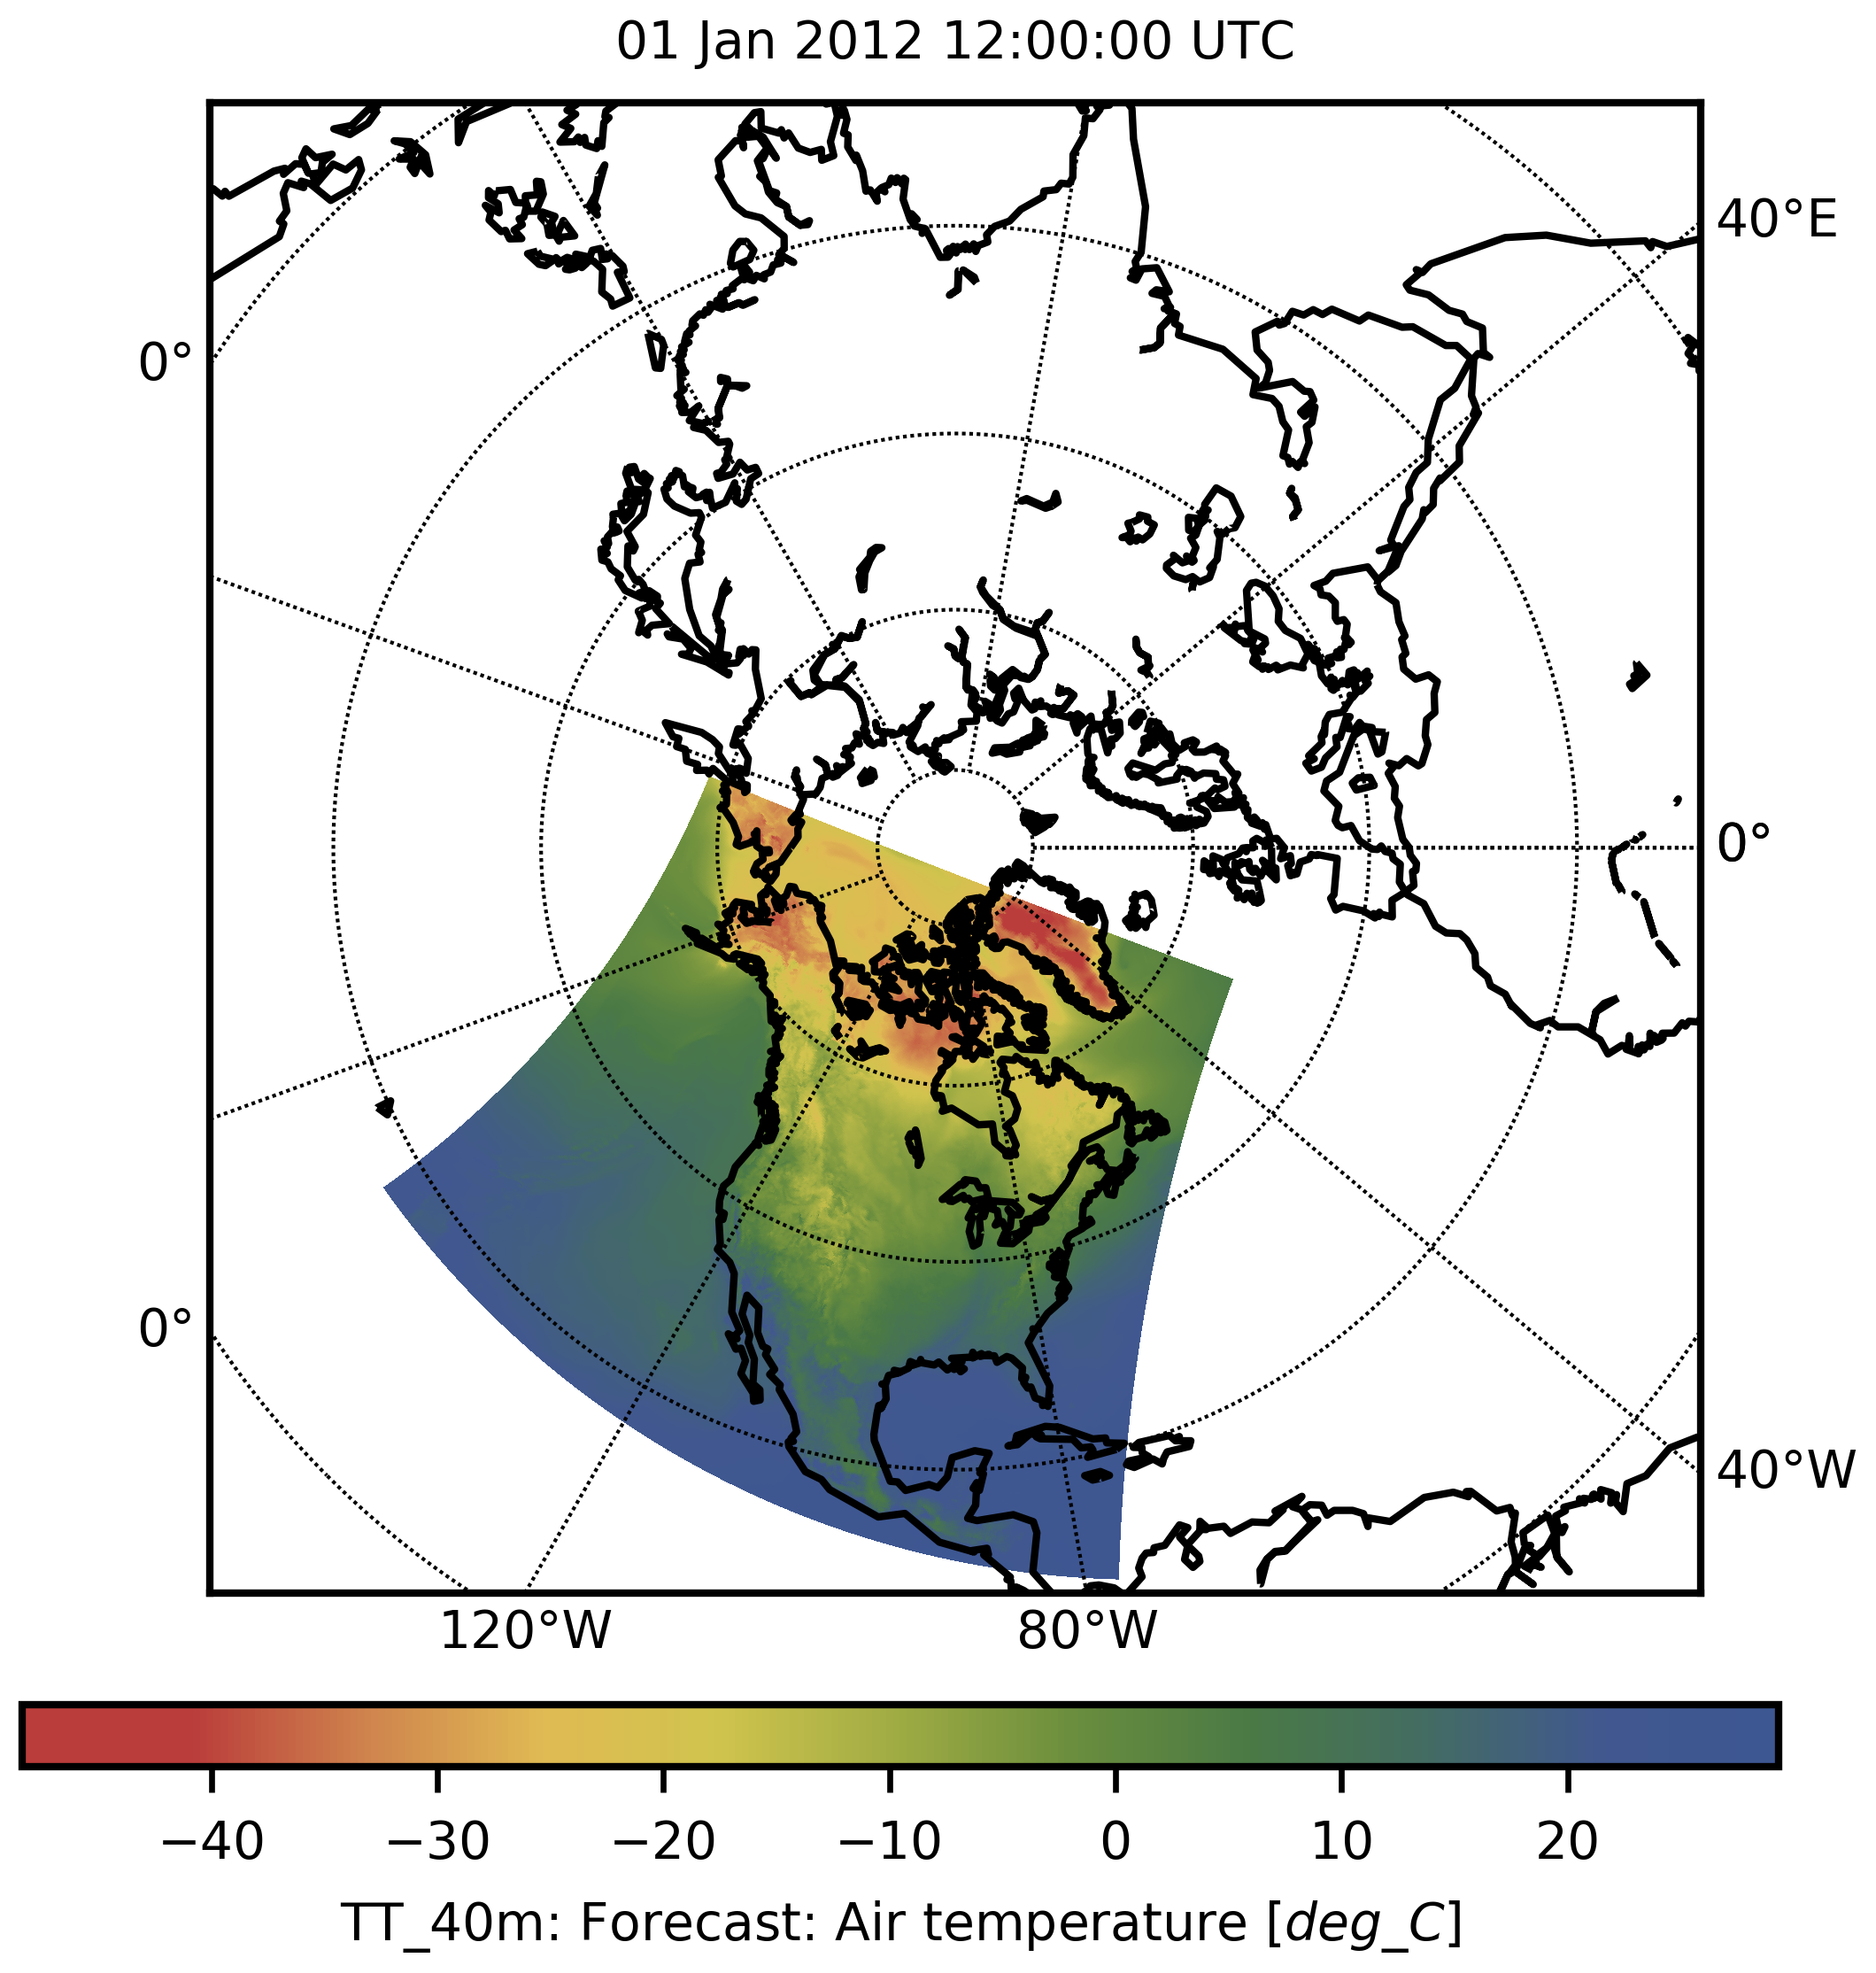
\includegraphics[width=0.45\linewidth]{figures/rdrs_domain.png}
		\caption{The Regional Deterministic Reforecast System (RDRS) dataset provided by ECCC-CMC~\citep{gasset2017c,gasset2018a} covers North America and parts of Central America. The plot shows as an example variable (temperature \texttt{TT\_40m}) at a randomly selected time step (2012-01-01 12:00 UTC noon). The spatial resolution of each RDRS variable is about 14.3~km. The temporal resolution is hourly spanning the period from Jan 1, 2010 12:00 UTC to Jan 1, 2015 12:00 UTC.}
		\label{fig:RDRS_domain}
	\end{figure}
	
	Five years of data (2010-01-01 12:00:00 UTC to 2015-01-01 12:00:00 UTC) have been provided at an hourly timestep covering North America and parts of Central America (see Figure~\ref{fig:RDRS_domain} for spatial coverage). Variables provided include all major forcings needed to run hydrologic and land-surface models (Table~\ref{tab:RDRS_variables}).
	Except for precipitation, all variables are outputs from 6-h to 18-h reforecast leadtime (not CaLDAS analysis) from the RDRS.  For its part, precipitation is based on the after-the-fact 24-h accumulation CaPA analysis that has been disaggregated on an hourly basis relying on the spatio-temporal evolution of precipitation from the RDRS 6-h to 18-h reforecast leadtime as well as on 6-h accumulation CaPA analysis achieved online. 
	
	\begin{table}[h!]
		\caption{Variables in the reforecast dataset provided by ECCC-CMC~\citep{gasset2017c,gasset2018a}. The forcings are either available at surface or 40 m height. The average spatial resolution is 14.3~km while the temporal resolution is 1~h. }
		\label{tab:RDRS_variables}
		\centering
		{\small \begin{tabular}{p{8pc} p{3pc} p{8pc} p{3pc} p{3pc} p{3pc}}
				\hline
				Variable & Var. name & Long name & Unit & Level \\ \hline
				Precipitation Rate  & PR0 & Quantity of precip. & [m] & SFC \\
				Air Temperature     & TT & Air temperature & [\textcelsius] & 40m \\
				Inc. Shortwave Rad. & FB & Downward solar flux & [W/m$^2$] & SFC \\
				Inc. Longwave Rad.  & FI & Surf. inc. infrared flux & [W/m$^2$] & SFC \\
				Atmospheric Pressure& P0 & Surface pressure & [mb] & SFC \\
				Specific Humidity   & HU & Specific humidity & [kg/kg] & 40m \\
				Wind Components     & UU, VV & U/V-comp. of wind (along grid X/Y) & [kts] & 40m \\
				Corr. Wind Components & UUC, VVC & U/V-comp. of wind (along W-E/S-N direct.) & [kts] & 40m \\
				Wind Speed & UVC & Wind modulus & [kts] & 40m \\
				Wind Direction & WDC & Meteorol. wind direction & [degree] & 40m \\ \hline
		\end{tabular}}
	\end{table}
	
	The 5-years dataset provided by ECCC-CMC is in FST format and was converted to NetCDF. Each day of the dataset was provided as a separate file following the name pattern \texttt{YYYYMMDD12.nc} specifying the issue date. Each file contains 25 time steps (YYYY-MM-DD 12:00, YYYY-MM-DD 13:00, YYYY-MM-DD 14:00, ..., YYYY-MM-DD+1 11:00, YYYY-MM-DD+1 12:00). For all variables except precipitation the first timestep of one file is the same as the last time step of the previous issue date. Precipitation is zero at the first timestep (YYYY-MM-DD 12:00). When files are merged, it is hence important to discard the first time step and keep the last timestep of each file. Also, as a side note, the sum of the 24 hourly accumulation of precipitation fields contained in a file produce exactly the original 24-h CaPA analysis.\\[4pt]	
	The shape of Lake Erie was downloaded from \url{https://www.sciencebase.gov/catalog/item/530f8a0ee4b0e7e46bd300dd} (see Figure~\ref{fig:LakeErie_maps}c) and used to crop the domain of Lake Erie (see Figure~\ref{fig:LakeErie_maps}d). All files of the RDRS dataset were merged to one single file which contains the domain of Lake Erie and all hourly timesteps of the 5 years, i.e. 2010-01-01 12:00 to 2015-01-01 12:00.
	
	\begin{figure}[h!]
		\centering
		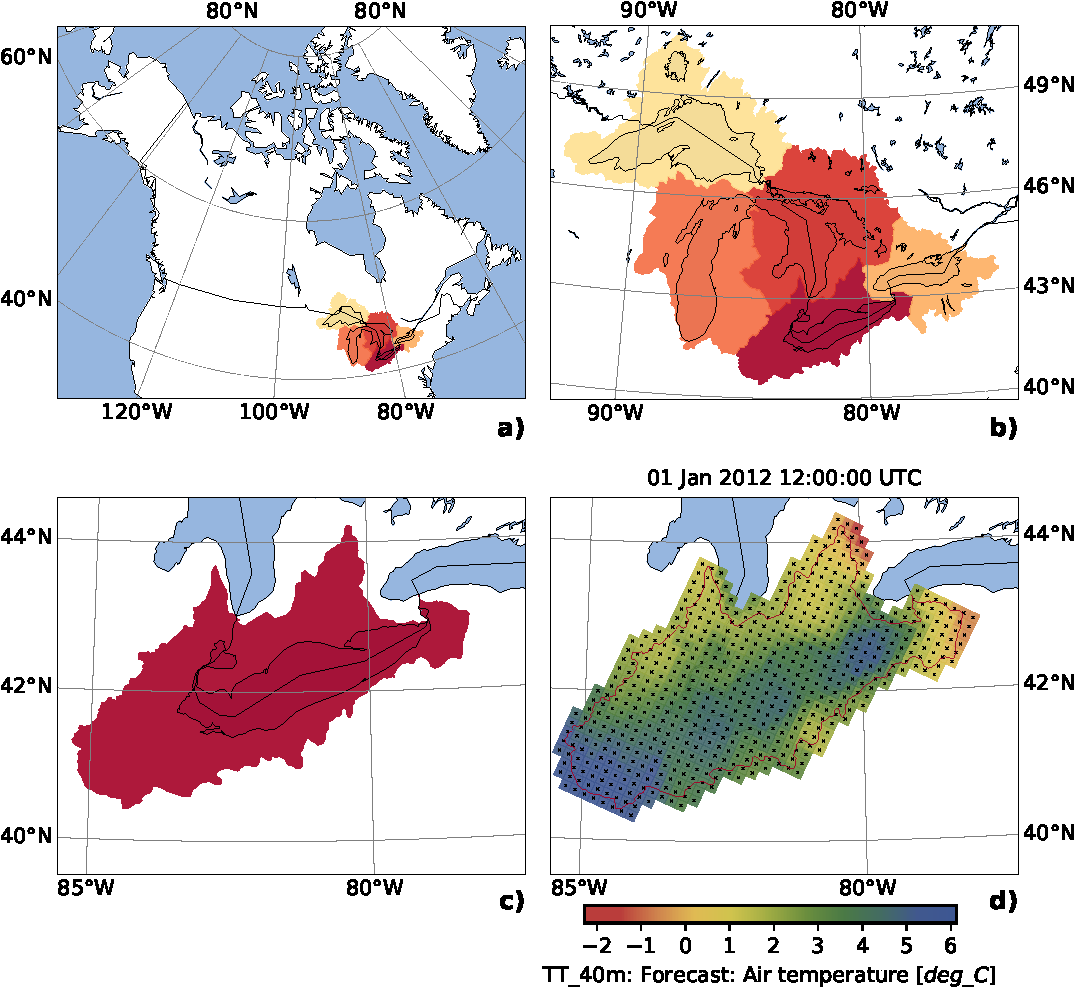
\includegraphics[width=0.75\linewidth]{figures/shapes_great_lakes.pdf}
		\caption{The location of the five color-coded Great Lakes (red: Lake Erie, dark-orange: Lake Huron, orange: Lake Michigan, light-orange: Lake Ontario, yellow: Lake Superior) as (a) an overview and (b) a close-up. (c) This study focuses on the domain of Lake Erie. (d) The domain of Lake Erie is cropped from the reforecast dataset provided by ECCC-CMC~\citep{gasset2017c,gasset2018a}. The last panel shows the temperature (\texttt{TT\_40m}) of a randomly selected time step (2012-01-01 12:00 UTC noon).}
		\label{fig:LakeErie_maps}
	\end{figure}
	

	\bibliography{references}
	
	
\end{document}	